\appendix
\section{Additional tables and figures}
\label{sec:appendix}

\subsection{Seed and draw conventions}
\label{app:seeds}

Displacement is a random draw of which exposed workers lose employment,
subject to occupation-group quotas proportional to employment times mean
exposure. Throughout the paper, three conventions apply. The scenario grid
(Figures~\ref{fig:griddisp}--\ref{fig:gridgini}, and their appendix
variants below), the decomposition in Figure~\ref{fig:decomp}, the preset
scenarios and the four incidence families are single draws at seed~0. The
decile transition and wage-gain profiles (Figures~\ref{fig:transition}
and~\ref{fig:wages}) are means over 50 independent draws. The robustness
summary and the confidence intervals in Figure~\ref{fig:decomp-ci} are
20-draw Monte Carlo runs, with $\pm$ values reported as standard deviations
across draws. Within each draw, ordering keys are uniform within occupation
group, so a record's inclusion probability does not depend on its grossing
weight.

\subsection{Job loss by occupation group}

Table~\ref{tab:jobloss} reports the central-scenario displacement rate for
each SOC2020 major group. The allocation rule concentrates losses in
administrative and secretarial work (10.5 per cent of the group's
employment), managerial and professional occupations (around 9.5 per cent)
and associate professional roles, while elementary occupations---the
least-exposed group, whose normalised exposure score is zero---experience
no displacement at all. Clerical and professional work bears the shock;
manual and elementary work is insulated.

\begin{table}[htbp]
\centering
\caption{Central-scenario job loss by SOC2020 major group}
\label{tab:jobloss}
\begin{tabular}{lrrr}
\toprule
Major group & C-AIOE & Employment (m) & Job loss (\%) \\
\midrule
1 Managers, directors and senior officials & 0.62 & 2.45 & 9.6 \\
2 Professional occupations & 0.60 & 6.46 & 9.5 \\
3 Associate professional occupations & 0.47 & 3.13 & 8.5 \\
4 Administrative and secretarial occupations & 0.74 & 2.35 & 10.5 \\
5 Skilled trades occupations & $-0.33$ & 1.56 & 2.8 \\
6 Caring, leisure and other service occupations & $-0.14$ & 2.32 & 3.9 \\
7 Sales and customer service occupations & 0.27 & 1.22 & 7.2 \\
8 Process, plant and machine operatives & $-0.54$ & 1.41 & 1.3 \\
9 Elementary occupations & $-0.73$ & 2.05 & 0.0 \\
\bottomrule
\end{tabular}

\vspace{2pt}
{\footnotesize C-AIOE is the standardised complementarity-adjusted exposure
score before the min-zero normalisation used in the allocation rule.
Employment and job-loss rates are survey-weighted; single draw, seed 0.}
\end{table}

\subsection{Where the shock lands: baseline distributions}

Figures~\ref{fig:b-market}--\ref{fig:b-disposable} show the baseline
household-level decile distributions of the income components through which
the three channels operate (aggregate \pounds billion per year by decile of
equivalised household disposable income). Market income excluding capital
(\pounds 1{,}313 billion in total) and income tax and National Insurance
(\pounds 312 billion) are heavily concentrated in the top deciles---which
is why displacement of high earners is fiscally expensive. Benefits
(\pounds 320 billion) are spread across the lower and middle deciles,
peaking in deciles~3 to~5. Capital income (\pounds 23 billion of interest
and dividends) is the most concentrated series of all: the top decile
holds more than a third of the total.

\begin{figure}[htbp]
\centering
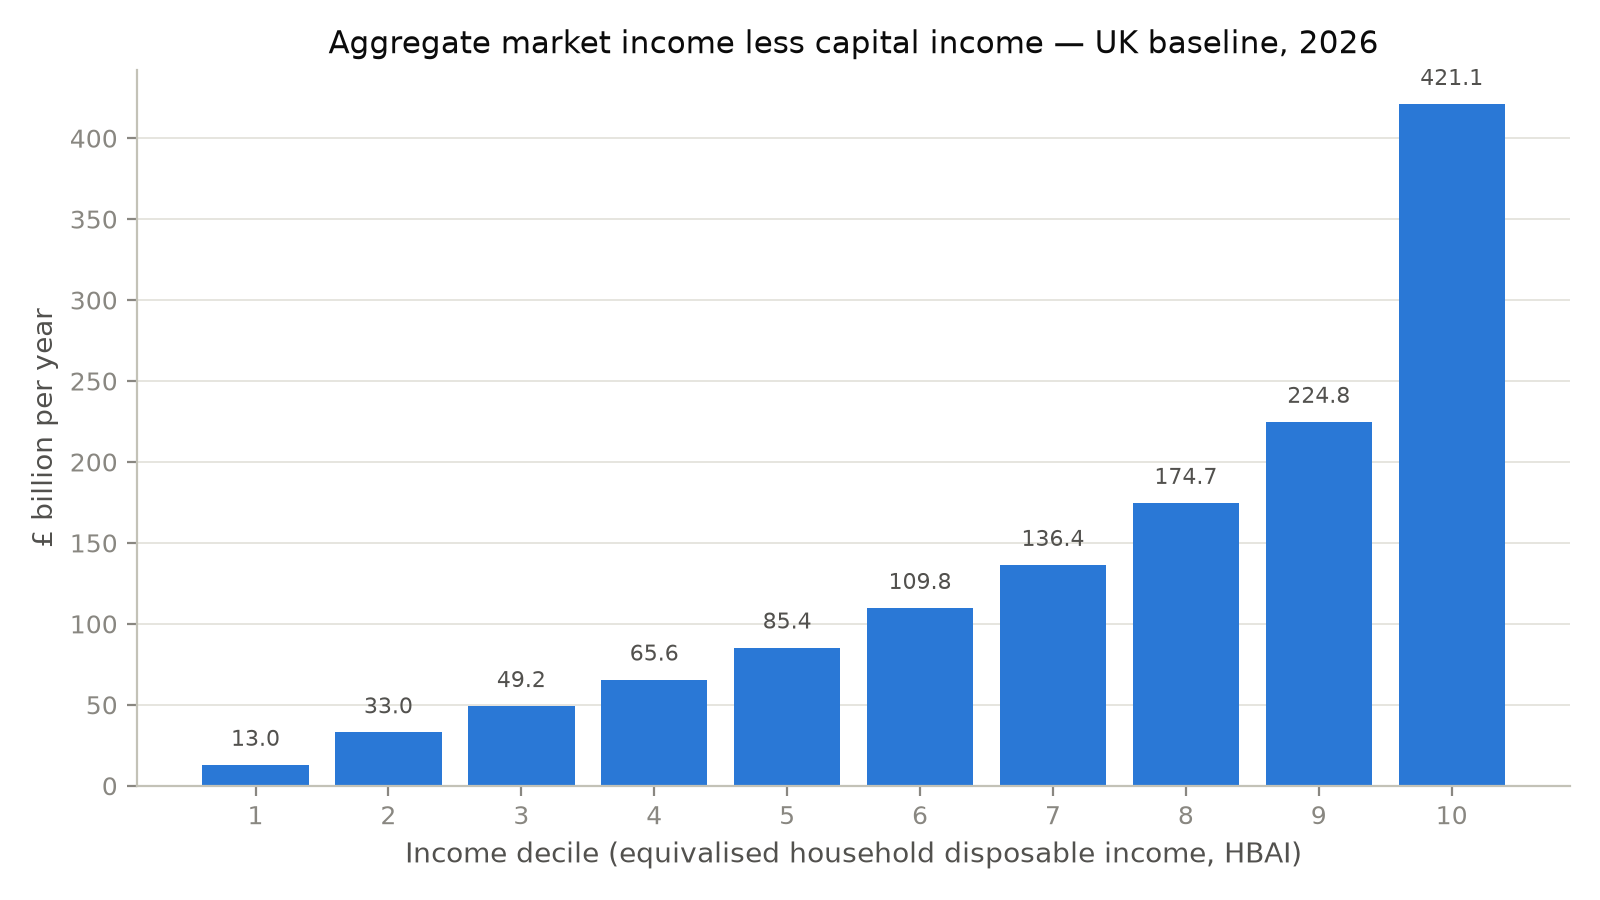
\includegraphics[width=.75\textwidth]{../results/appendix/b1_market_income_less_capital.png}
\caption{Baseline aggregate household market income (less capital income) by decile.}
\label{fig:b-market}
\end{figure}

\begin{figure}[htbp]
\centering
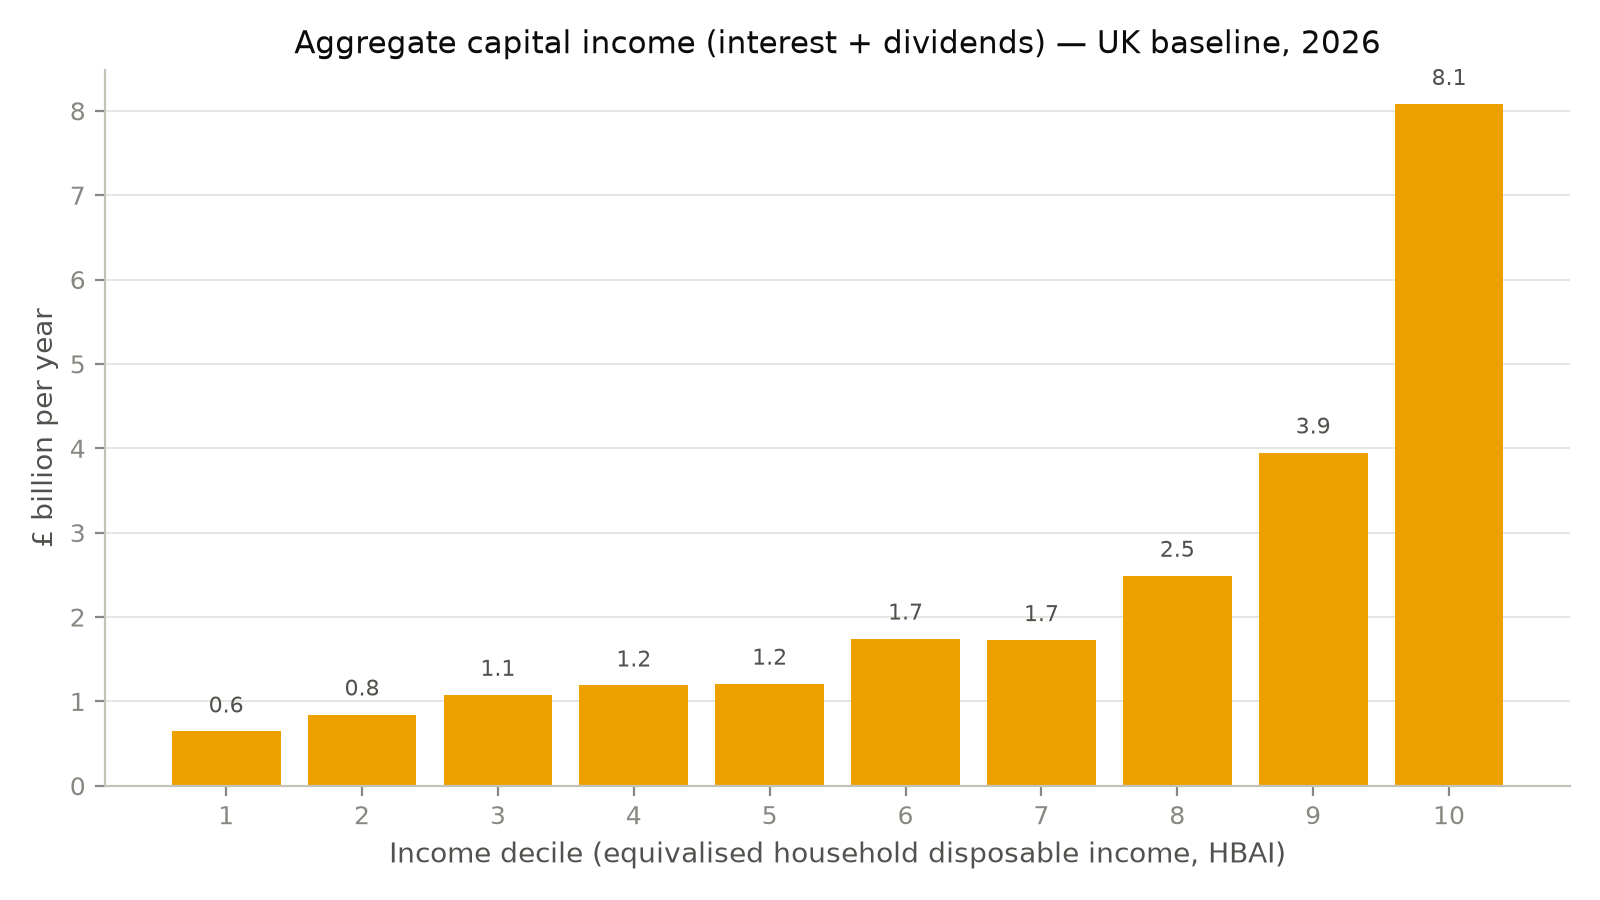
\includegraphics[width=.75\textwidth]{../results/appendix/b2_capital_income.png}
\caption{Baseline aggregate household capital income (interest and dividends) by decile.}
\label{fig:b-capital}
\end{figure}

\begin{figure}[htbp]
\centering
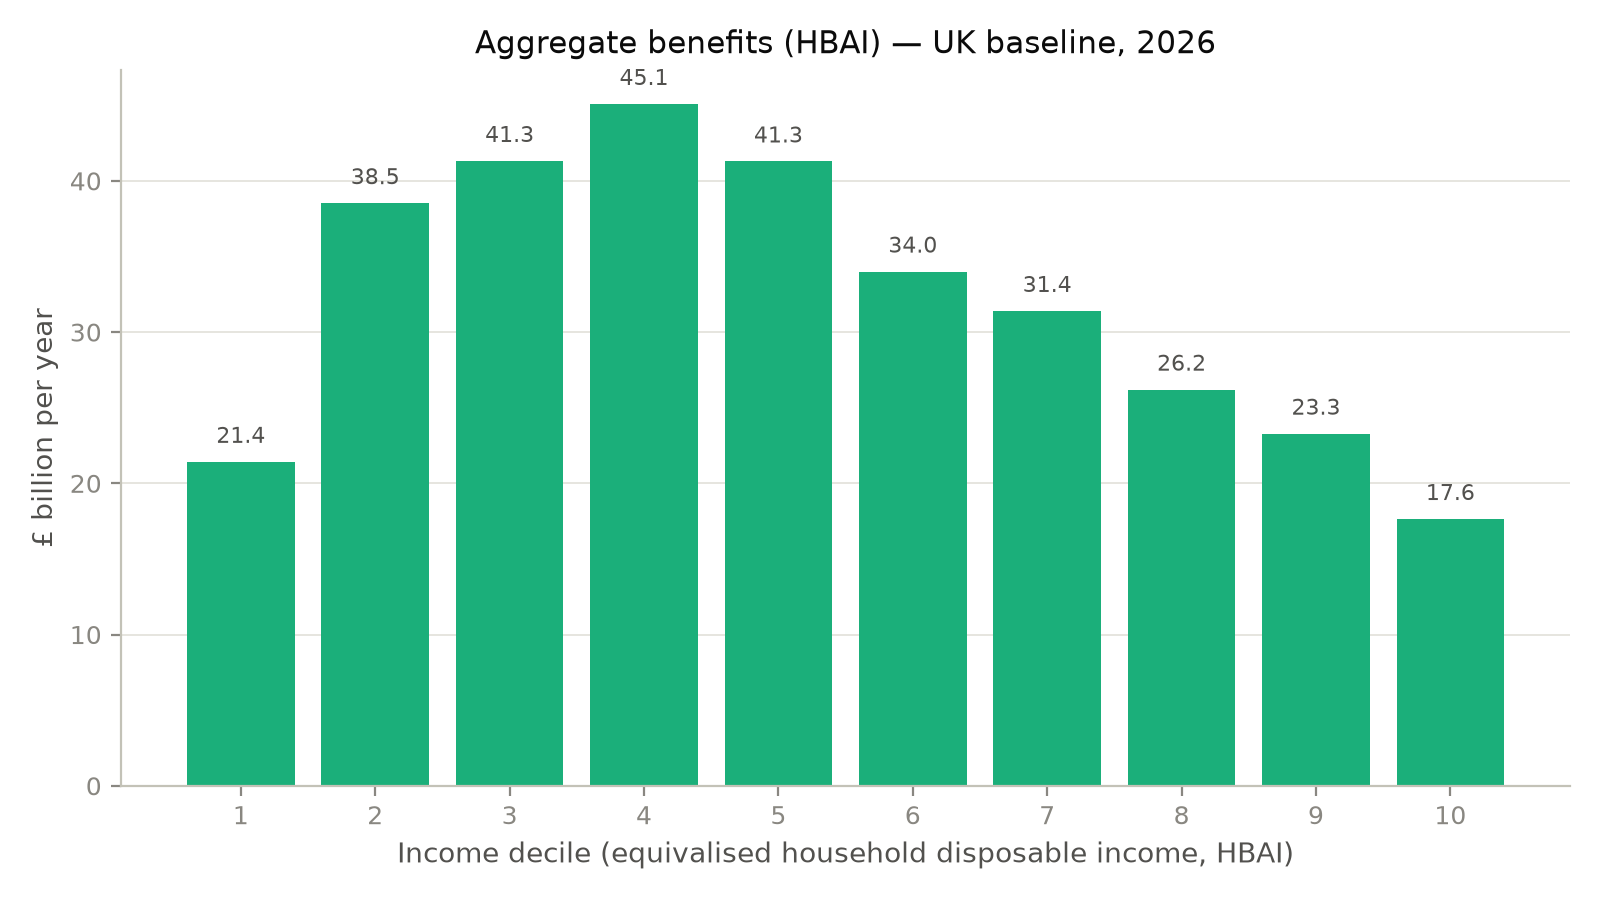
\includegraphics[width=.75\textwidth]{../results/appendix/b3_benefits.png}
\caption{Baseline aggregate household benefits by decile.}
\label{fig:b-benefits}
\end{figure}

\begin{figure}[htbp]
\centering
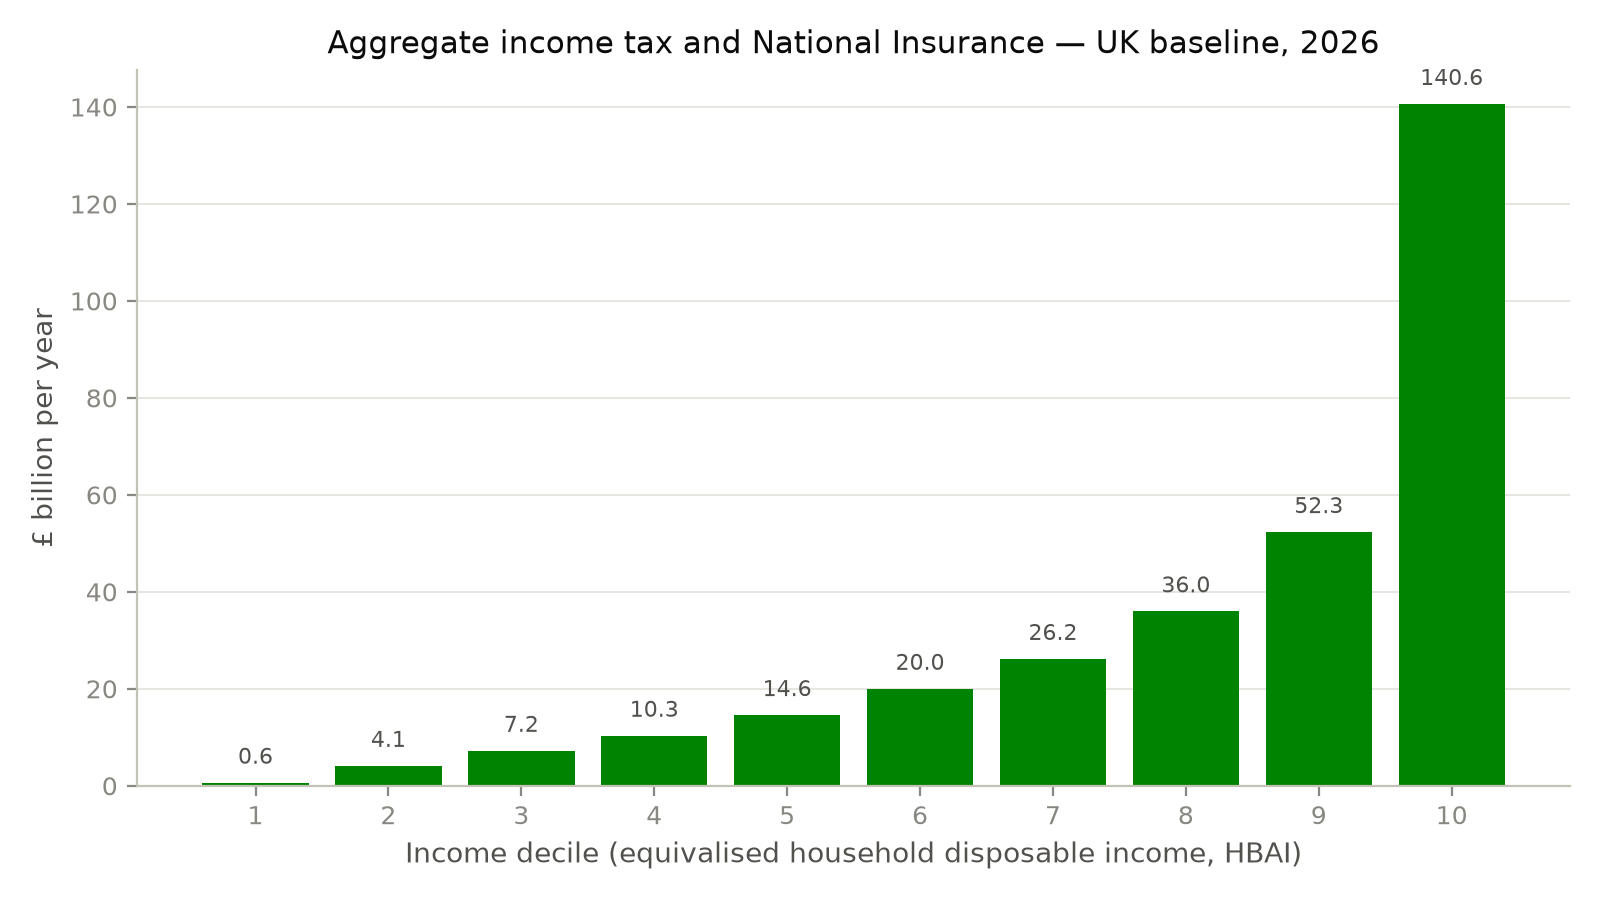
\includegraphics[width=.75\textwidth]{../results/appendix/b4_tax_and_ni.png}
\caption{Baseline aggregate household income tax and National Insurance by decile.}
\label{fig:b-tax}
\end{figure}

\begin{figure}[htbp]
\centering
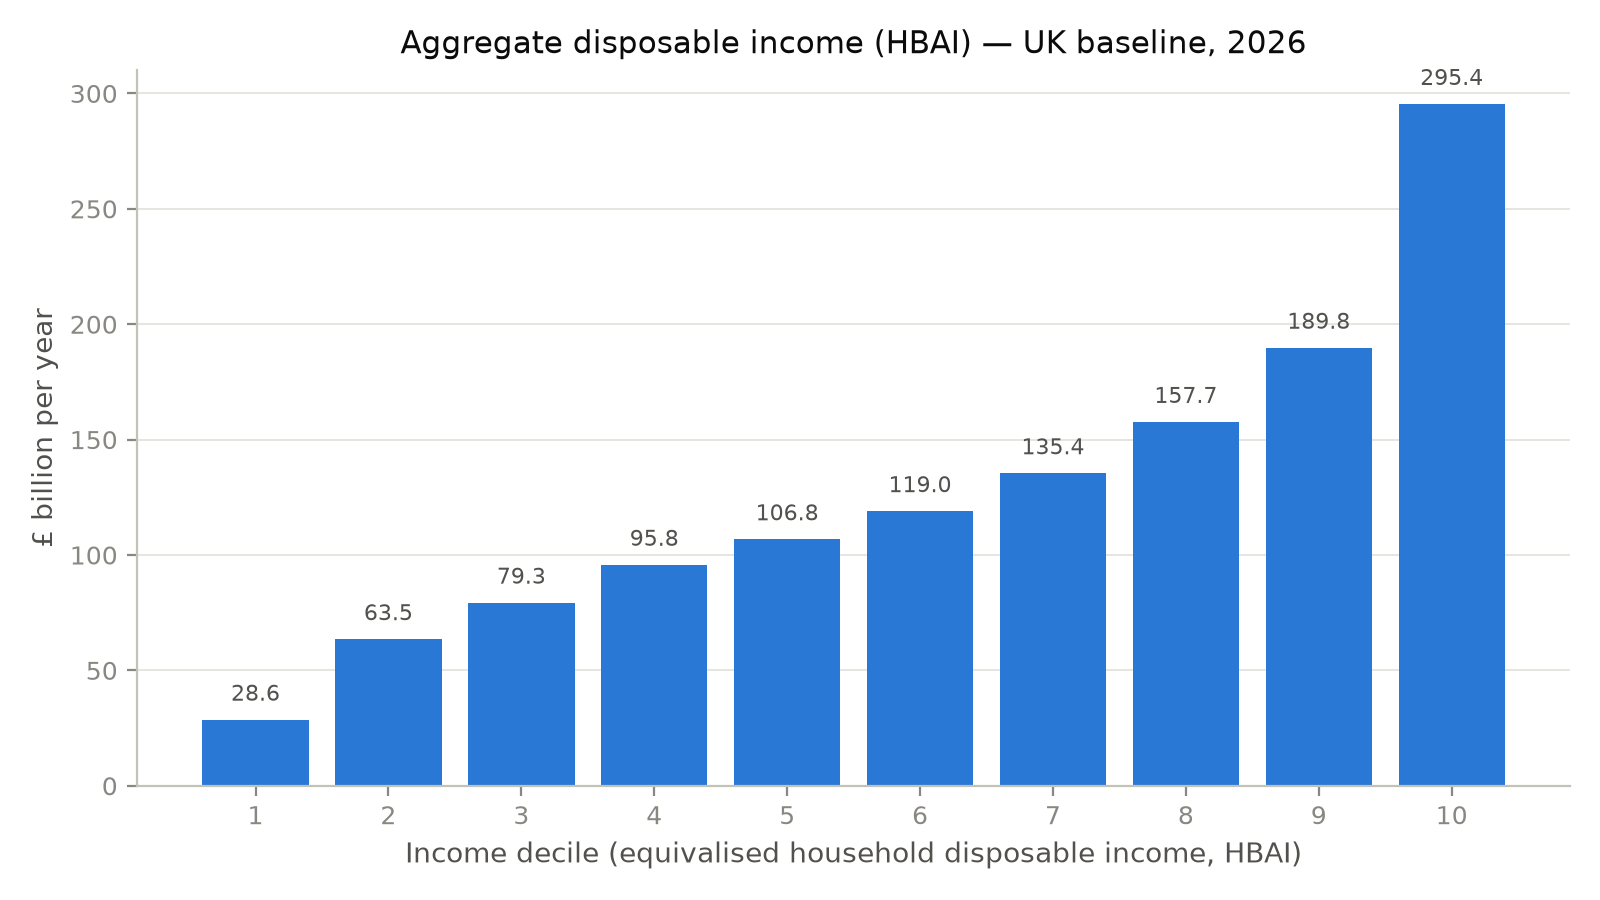
\includegraphics[width=.75\textwidth]{../results/appendix/b5_disposable_income.png}
\caption{Baseline aggregate household disposable income (HBAI concept) by decile.}
\label{fig:b-disposable}
\end{figure}

\subsection{Exposure incidence before any simulation}

Figures~\ref{fig:exp-incidence} and \ref{fig:comp-incidence} show, without
any shock, how workers in each income decile distribute across
employment-weighted tertiles of AI exposure and of complementarity. The
share of workers in the top exposure tertile rises steadily with household
income, while complementarity shows no comparable gradient---the
descriptive facts that generate the simulated incidence in
Section~\ref{sec:results}.

\begin{figure}[htbp]
\centering
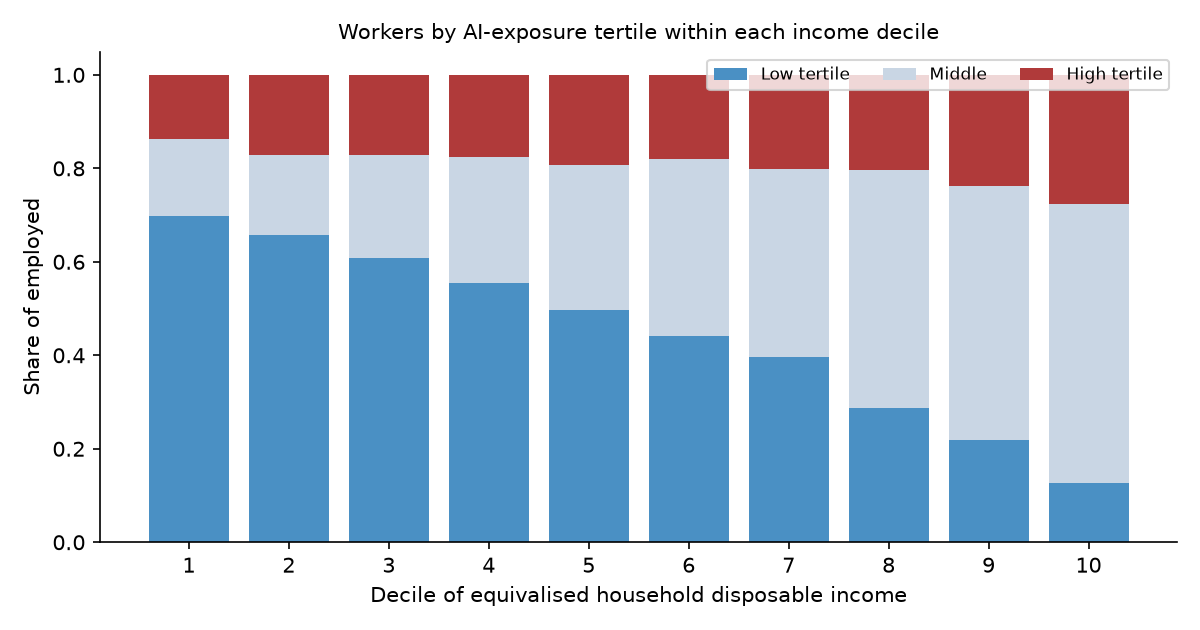
\includegraphics[width=.8\textwidth]{../results/appendix/exposure_incidence_by_decile.png}
\caption{Distribution of employed persons across AI-exposure tertiles, by income decile.}
\label{fig:exp-incidence}
\end{figure}

\begin{figure}[htbp]
\centering
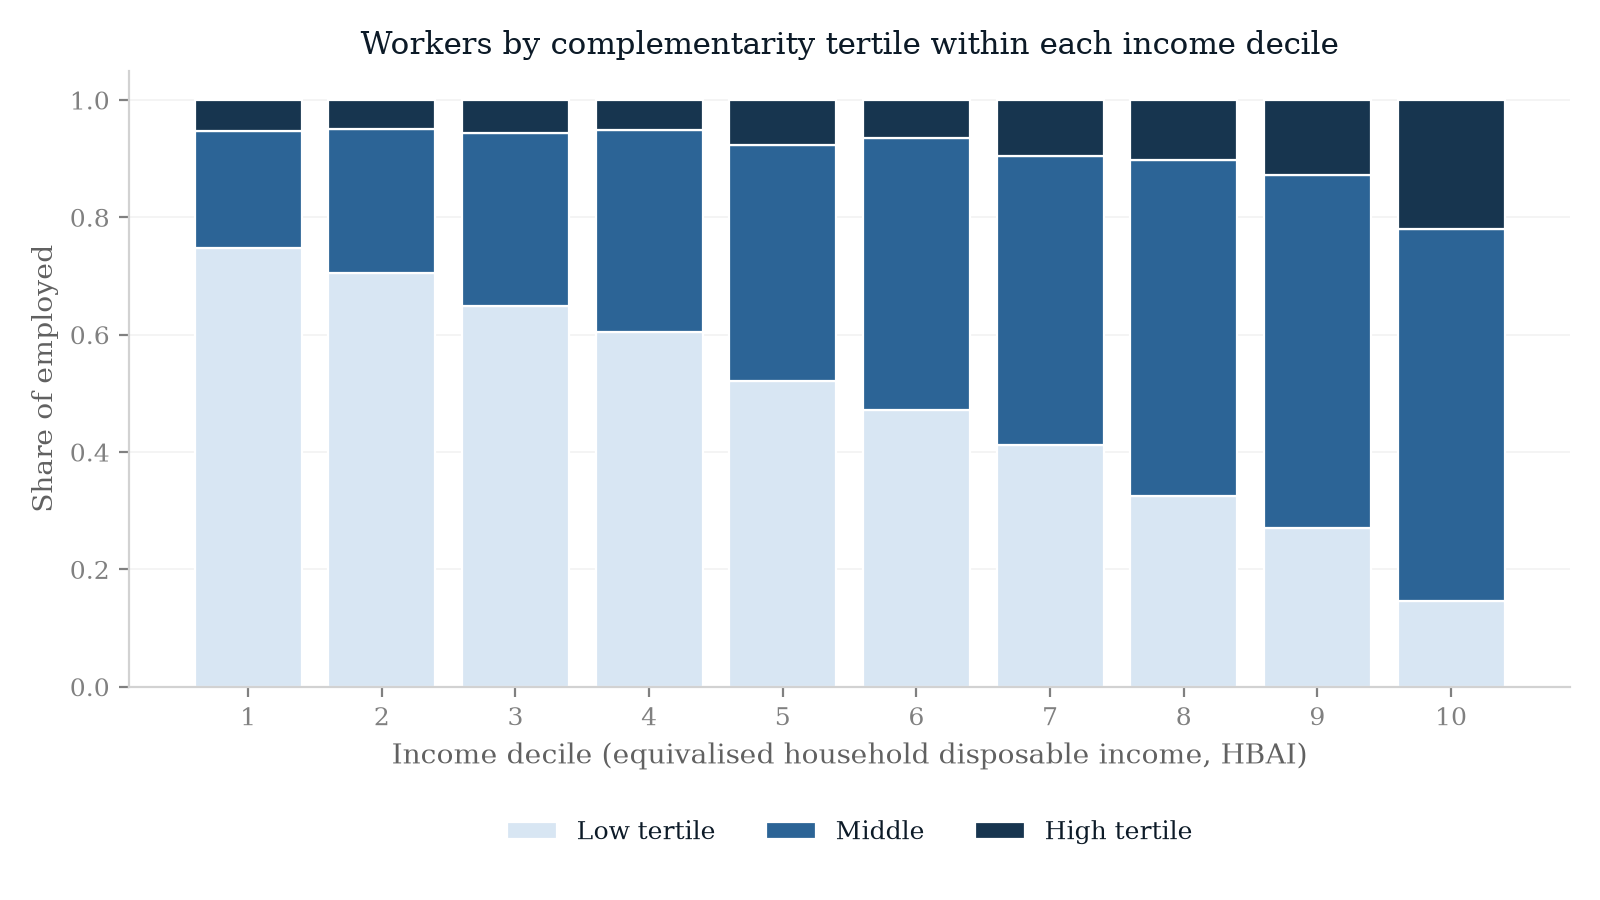
\includegraphics[width=.8\textwidth]{../results/appendix/complementarity_incidence_by_decile.png}
\caption{Distribution of employed persons across complementarity tertiles, by income decile.}
\label{fig:comp-incidence}
\end{figure}

\subsection{Monte Carlo uncertainty on the decile profile}

Figure~\ref{fig:decomp-ci} reports the central-scenario disposable-income
change by decile as the mean over twenty independent displacement draws
with 95 per cent confidence intervals. The gradient runs from $-0.5$ per
cent in the bottom decile to $-4.1$ per cent in the top. It is not quite
monotone: deciles~2 and~3 show a small reversal ($-0.88$ against $-0.82$
per cent), well inside the draw noise. The overall upward slope of the loss
profile survives the uncertainty comfortably.

\begin{figure}[htbp]
\centering
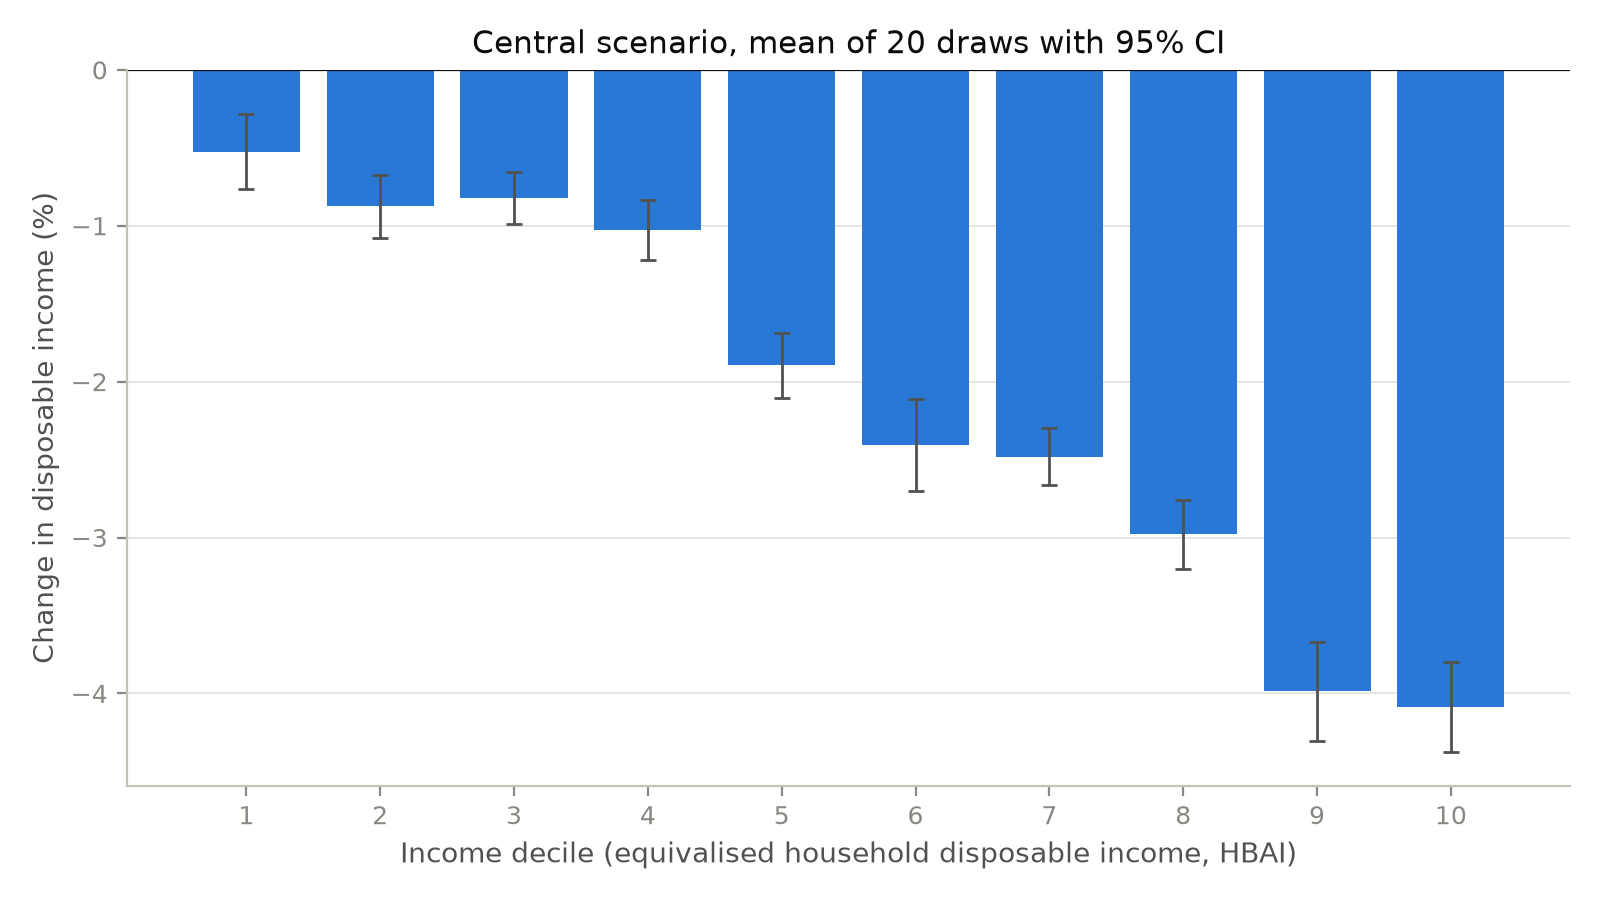
\includegraphics[width=.8\textwidth]{../results/appendix/decomposition_ci.png}
\caption{Disposable income change by decile, central scenario: mean of 20 displacement draws with 95 per cent confidence intervals.}
\label{fig:decomp-ci}
\end{figure}

\subsection{Uniform-shock and alternative-index comparisons by decile}

Figure~\ref{fig:b7} compares the central scenario against the same
aggregate shocks allocated uniformly across occupations, decile by decile;
Figure~\ref{fig:b8} repeats the central scenario with the
\citet{eloundou2023} GPT-exposure index in place of the C-AIOE. The
exposure-based allocation shifts losses up the distribution relative to a
uniform shock (top-decile losses of 3.9 against 3.0 per cent; bottom-decile
losses of 0.5 against 0.9 per cent), and the choice of exposure index
leaves the decile profile essentially unchanged.

\begin{figure}[htbp]
\centering
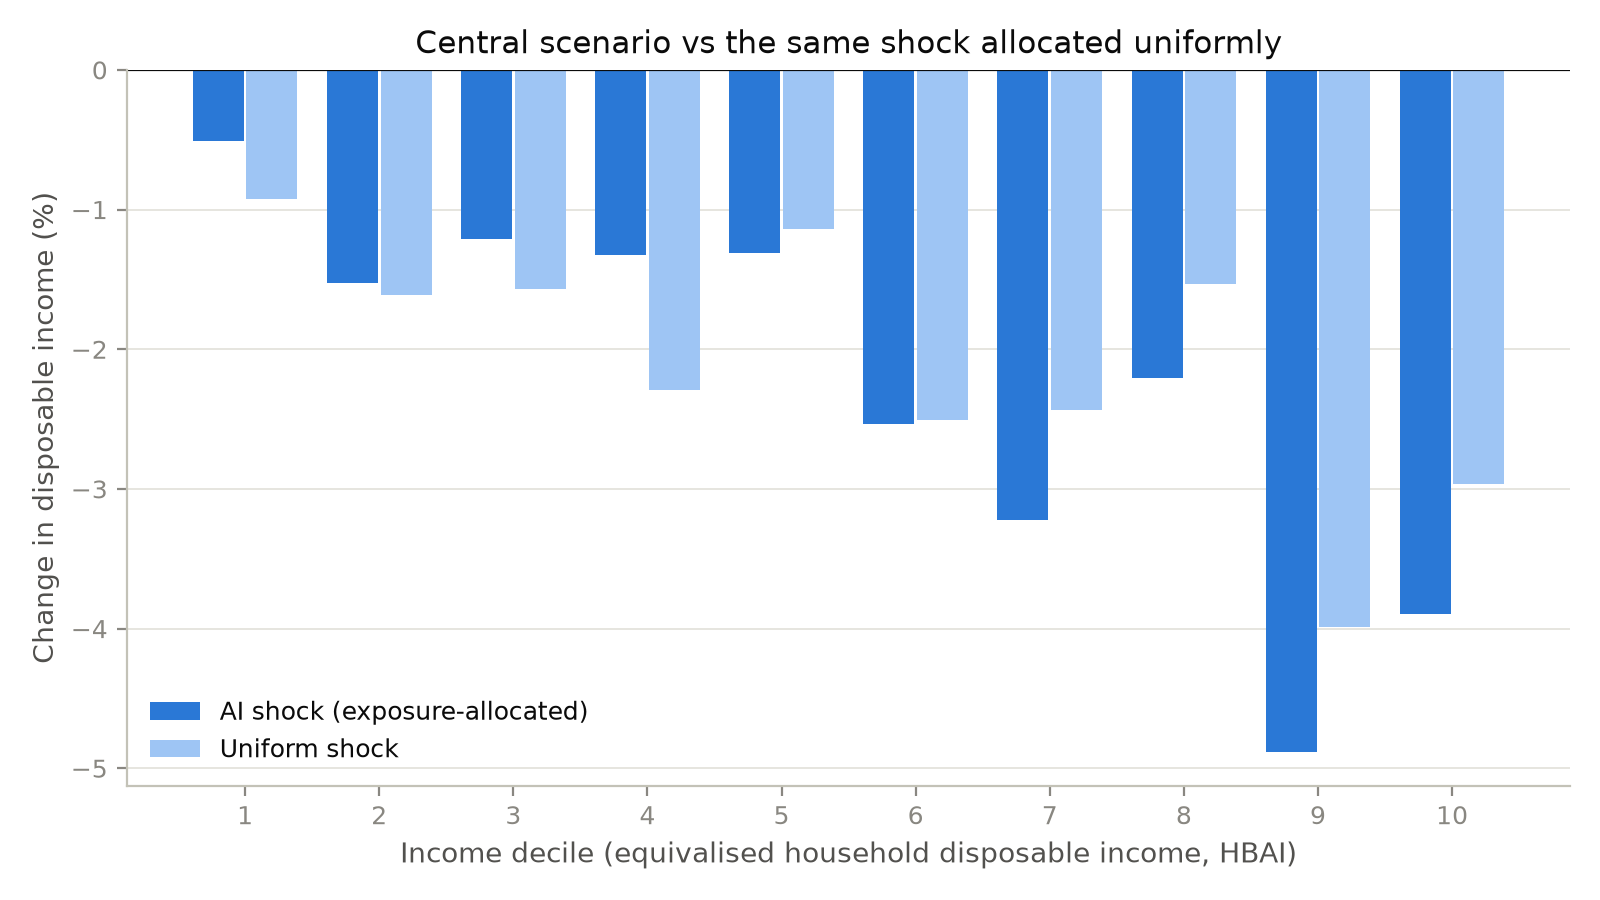
\includegraphics[width=.8\textwidth]{../results/appendix/b7_uniform_vs_ai_decile.png}
\caption{Disposable income change by decile: exposure-allocated versus uniform shock, central parameters.}
\label{fig:b7}
\end{figure}

\begin{figure}[htbp]
\centering
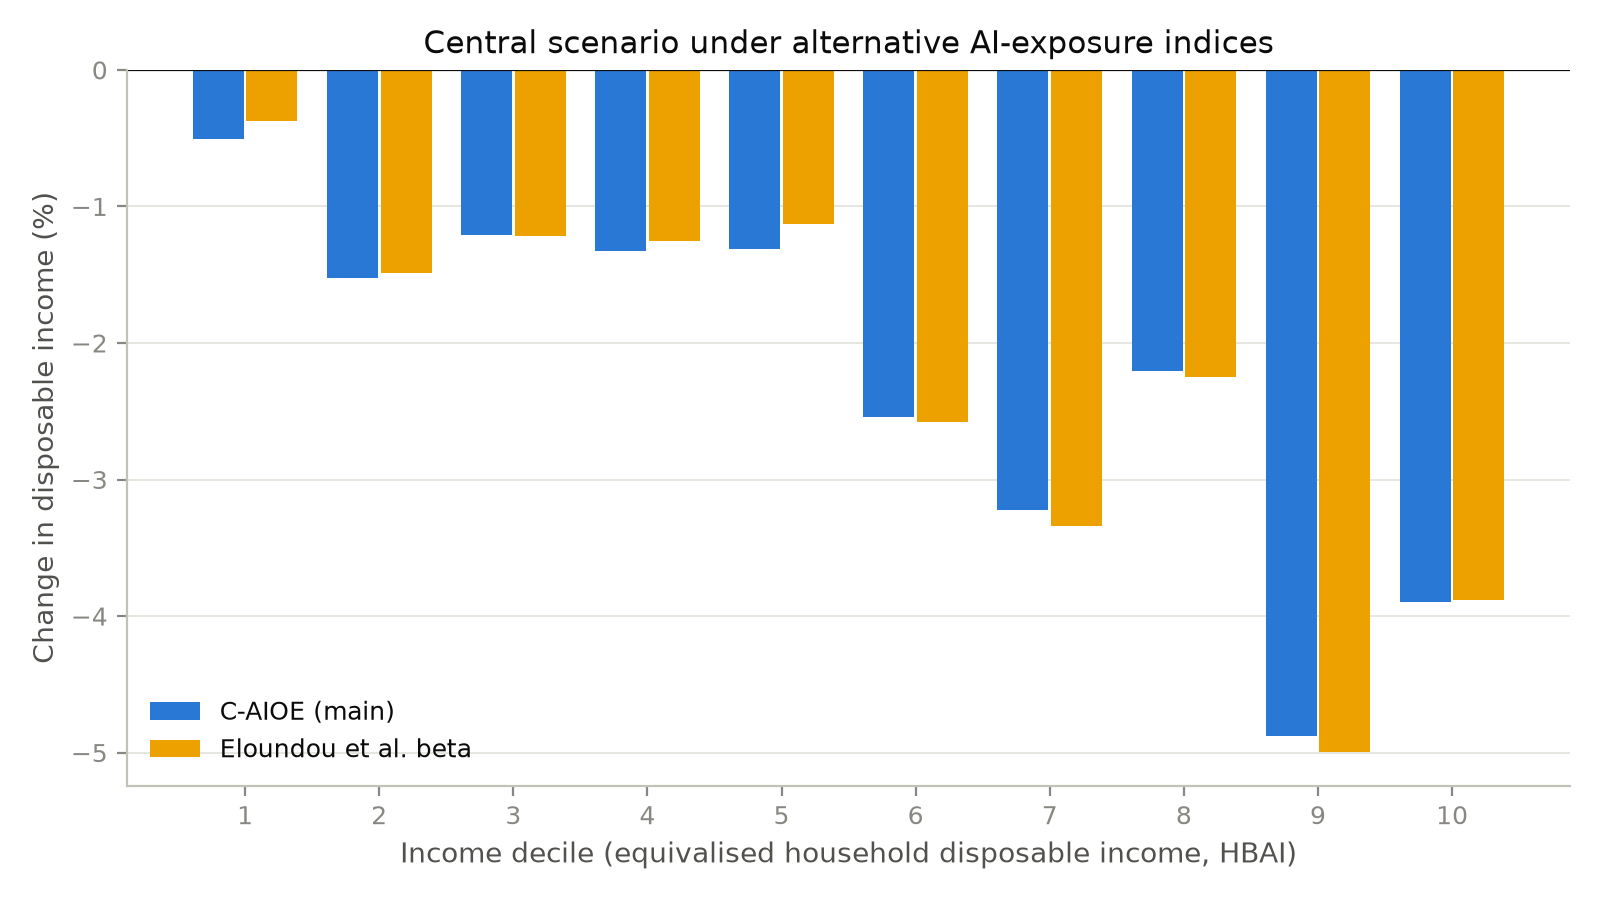
\includegraphics[width=.8\textwidth]{../results/appendix/b8_alternative_index_decile.png}
\caption{Disposable income change by decile under the C-AIOE and the Eloundou et al.\ exposure index.}
\label{fig:b8}
\end{figure}

\subsection{The scenario grid by decile, and without the capital shock}

Figure~\ref{fig:b9} facets the full 66-cell scenario grid by baseline
income decile; cells report the change in mean household disposable income
(HBAI concept), which across the grid as a whole ranges from $+3.0$ to
$-5.2$ per cent. Every decile's panel shifts towards losses as displacement
rises, but the top deciles darken much faster: in the harshest cell (10 per
cent displacement, no wage gain) the bottom decile loses 1.9 per cent of
disposable income while the top decile loses 8.2 per cent.
Figure~\ref{fig:b11} removes the capital-return shock. Average disposable
incomes fall relative to the capital-on grid, confirming that the capital
channel raises average incomes while concentrating its gains at the top;
the Gini result, however, is unchanged in kind: without the capital shock
the Gini of equivalised disposable income still rises in all 66 cells, by
0.00 to 1.50 percentage points. The inequality result does not depend on
the capital channel.

\begin{figure}[htbp]
\centering
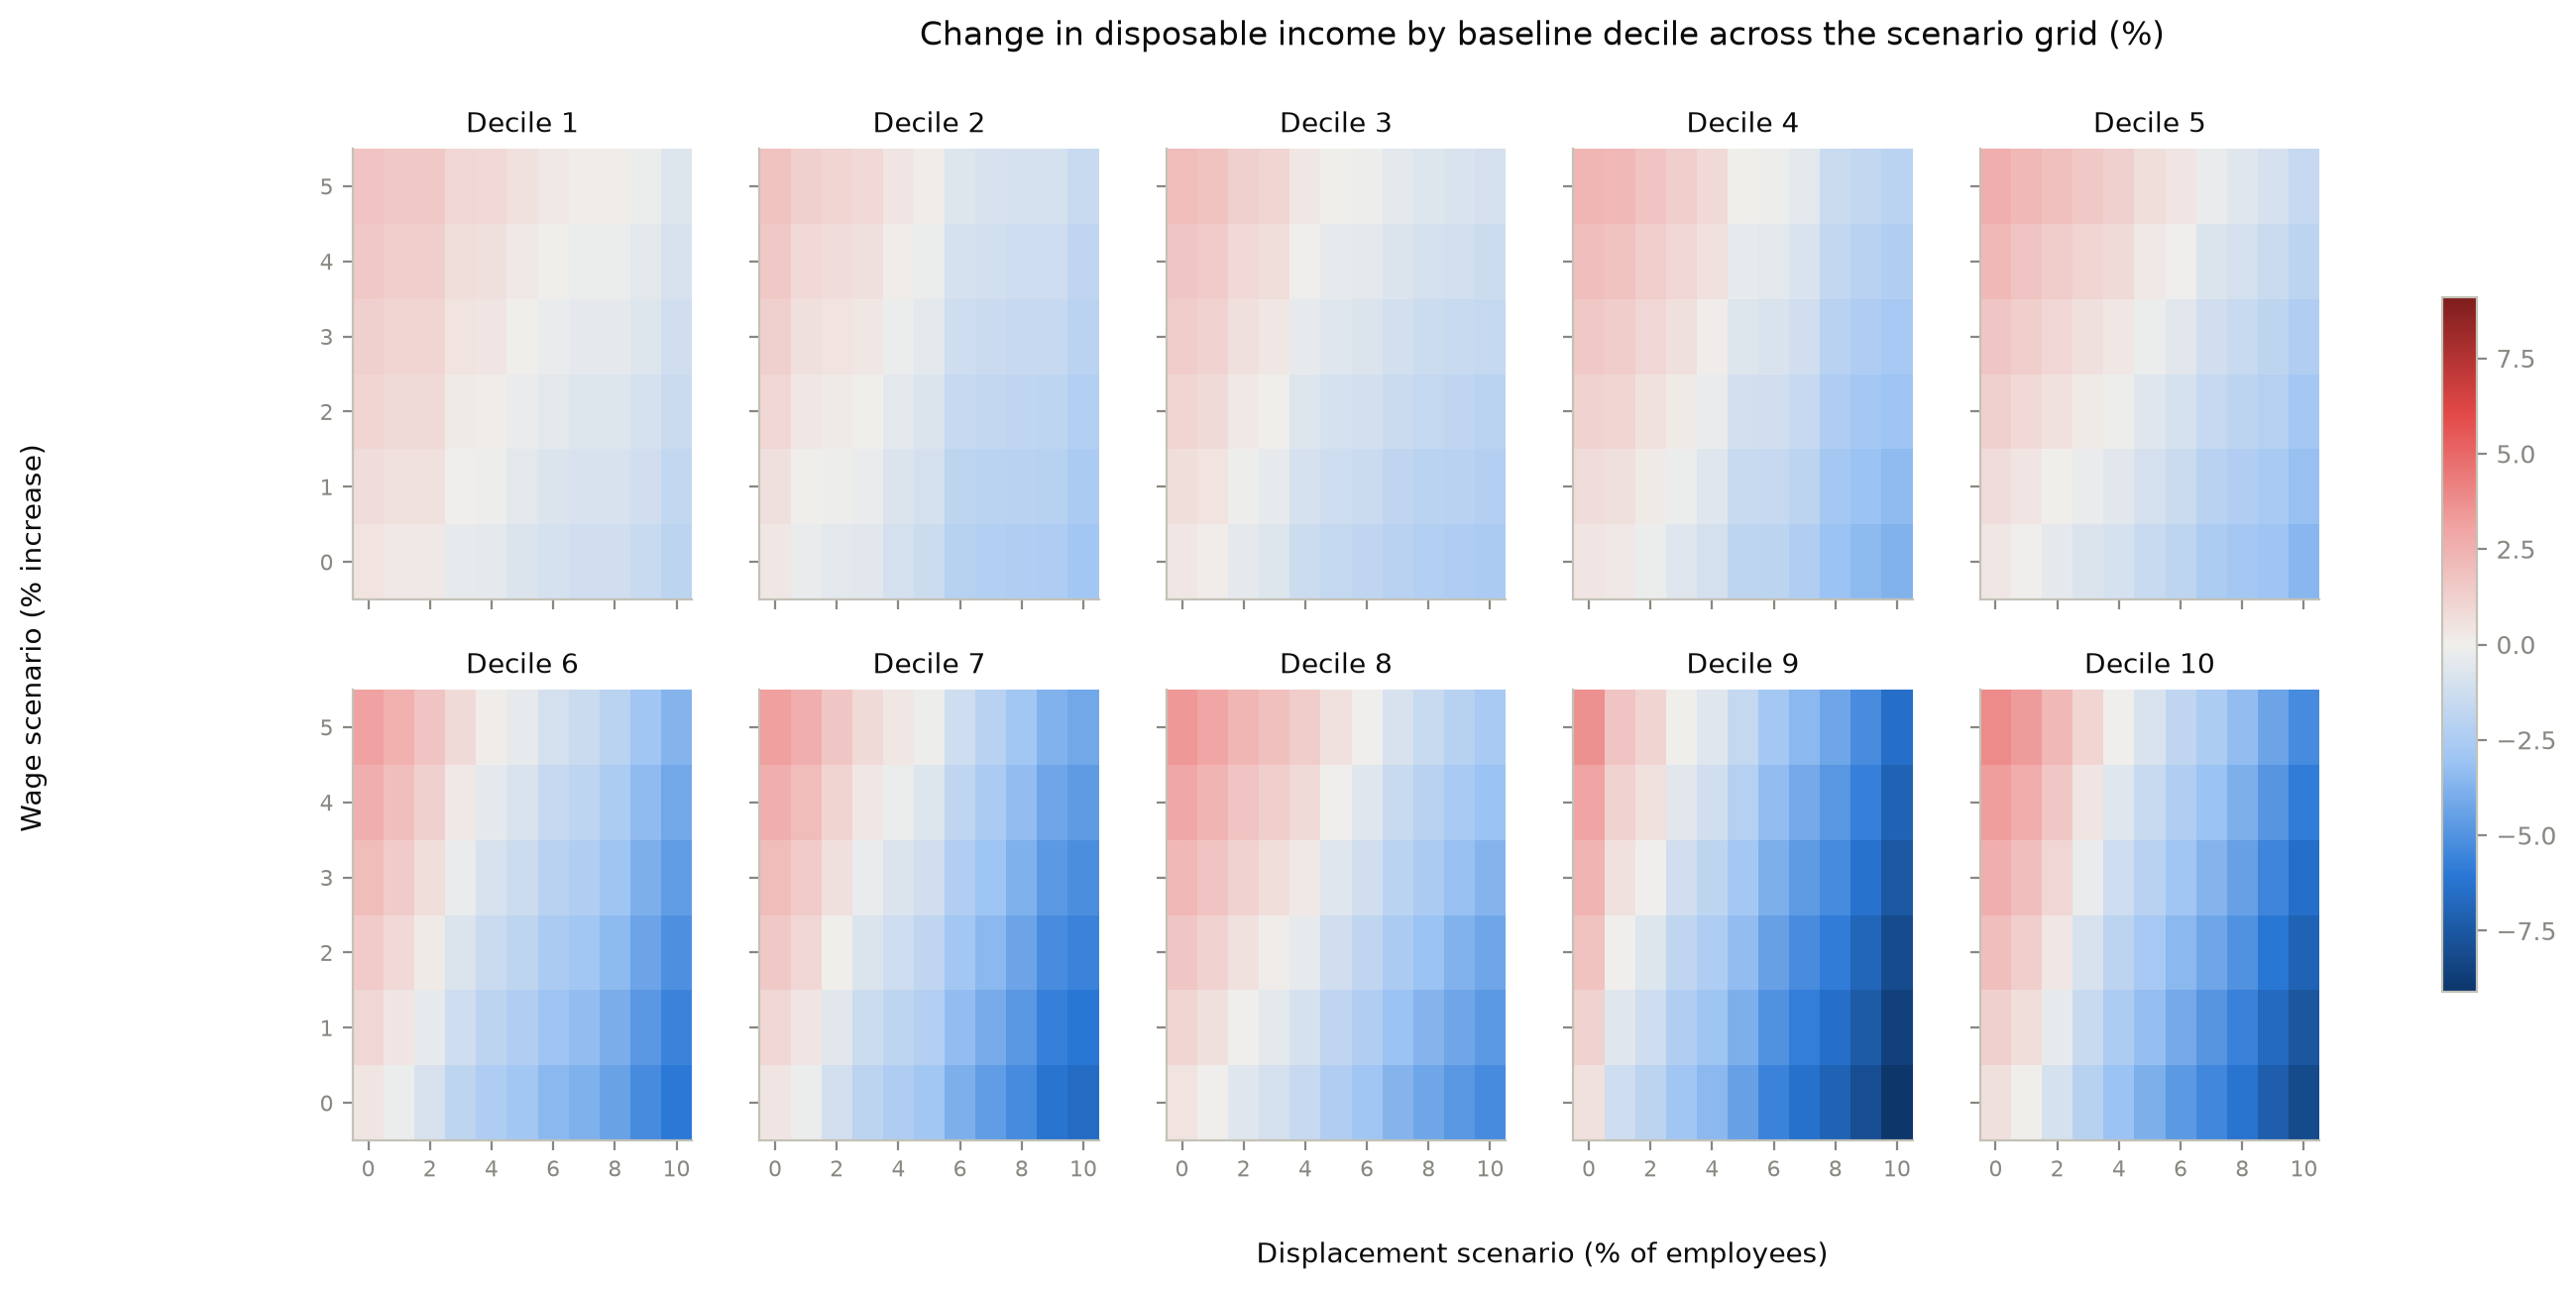
\includegraphics[width=\textwidth]{../results/appendix/b9_grid_by_decile.png}
\caption{Change in household disposable income across the scenario grid, faceted by baseline income decile. Single draw, seed 0.}
\label{fig:b9}
\end{figure}

\begin{figure}[htbp]
\centering
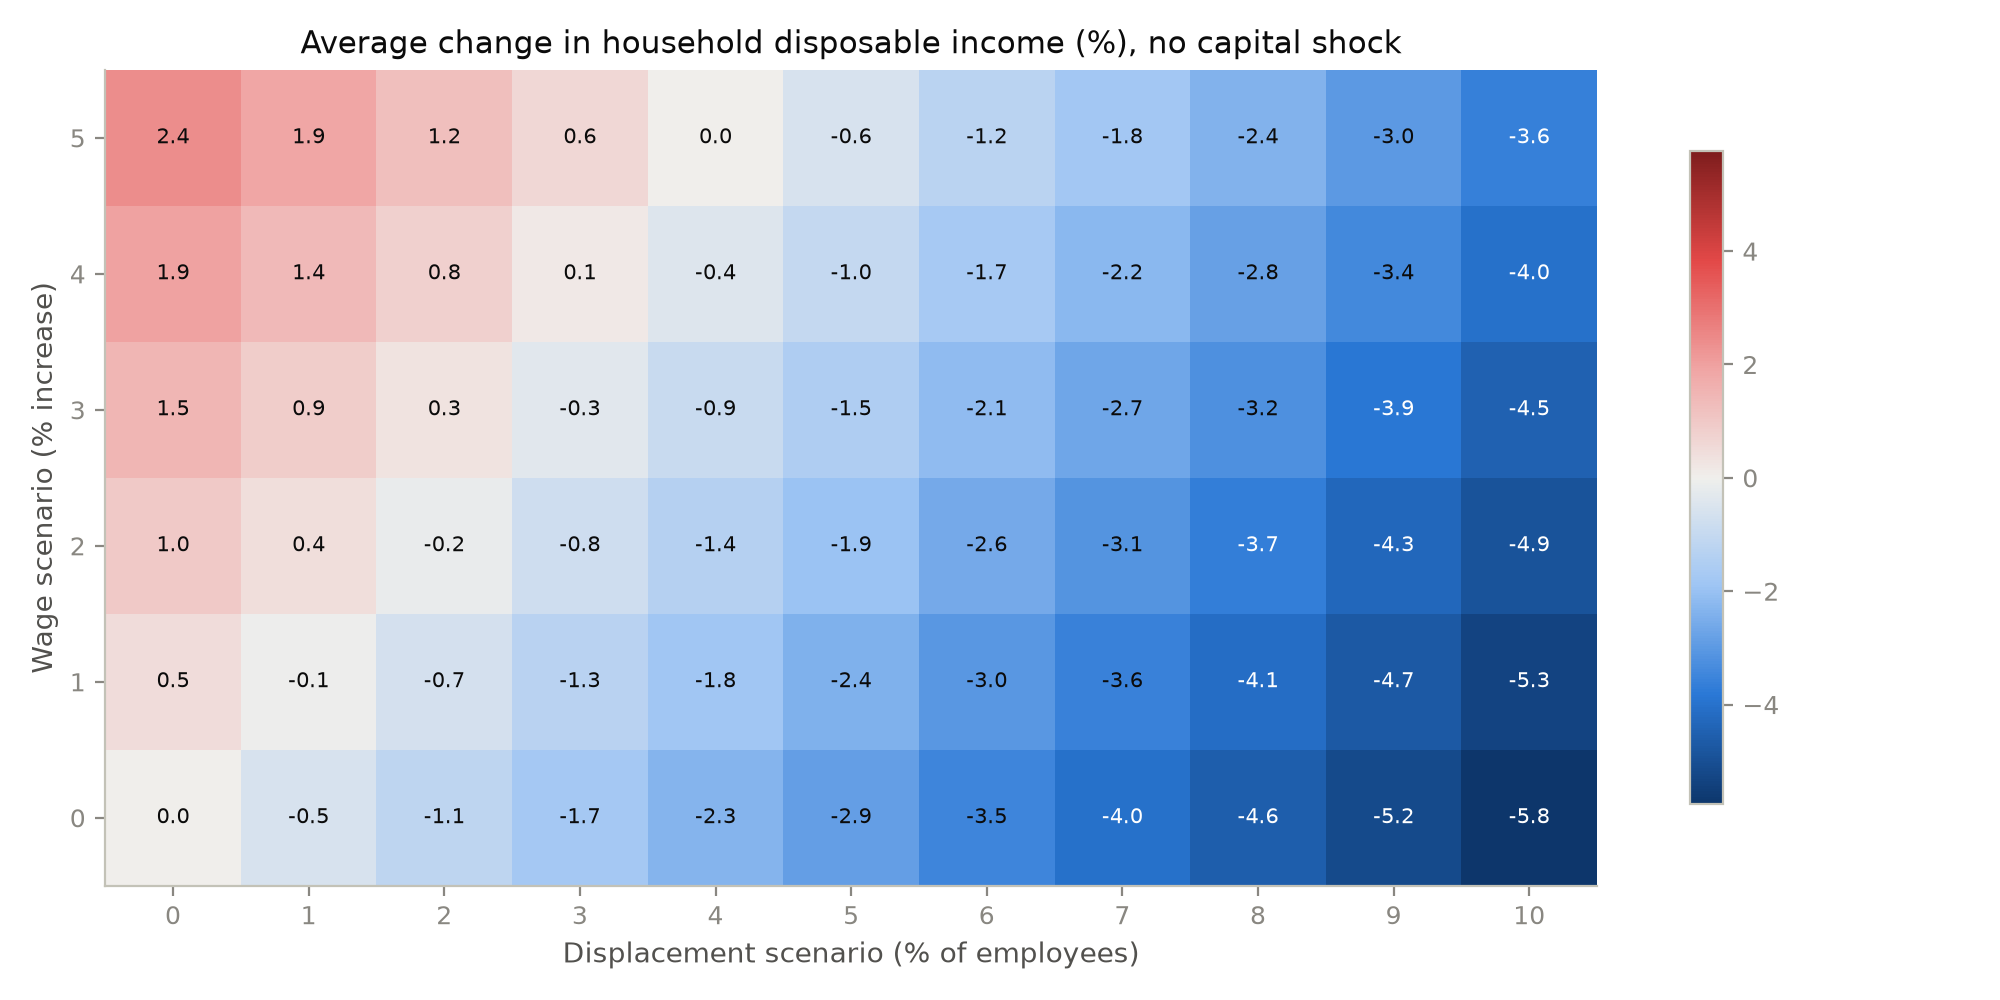
\includegraphics[width=.85\textwidth]{../results/appendix/b11_grid_no_capital.png}
\caption{Average change in household disposable income across the scenario grid with the capital-return shock switched off. Single draw, seed 0.}
\label{fig:b11}
\end{figure}
